\documentclass[a4paper, 11pt]{article}

%% Language and font encodings
\usepackage[english]{babel}
\usepackage[utf8x]{inputenc}
\usepackage[T1]{fontenc}
\usepackage{booktabs}

%% Sets page size and margins
\usepackage[a4paper,top=3cm,bottom=2cm,left=3cm,right=3cm,marginparwidth=1.75cm]{geometry}

%% Useful packages
\usepackage{amsmath}
\usepackage{graphicx}
\usepackage[colorinlistoftodos]{todonotes}
\usepackage[colorlinks=true, allcolors=blue]{hyperref}

\title{Local Geomagnetic Effects associated to strong Geomagnetic storms at Mexico’s Geomagnetic Latitude }
\author{Castellanos-Velazco, C. I., Corona-Romero, P., González-Esparza, J. A., Caccavari-Garza, A. L.}
\date{}

\begin{document}
\maketitle  
\begin{abstract}
The purpose of this project is to identify and characterize geomagnetic local effects on the center of Mexico during geomagnetic storms periods for the last two solar cycles. To identify such effects, we compare the planetary geomagnetic response (Dst index) and local geomagnetic response ($\mathrm{\Delta H}$ index) for the selected study cases. It was found out that a local geomagnetic response is presented  with Dst <-50 nT. It is important to consider that such local effects where systematically associated to local ionospheric disturbances.\\


\end{abstract}

\section*{Introduction}

Space Weather is defined as the conditions presented in the sun, interplanetary environment, solar wind,  magnetosphere, thermosphere and ionosphere. Solar magnetic activity has a strong influence on the behavior of the Earth’s magnetic field (EMF). When a disturbance is produced on the solar atmosphere, it propagates through the interplanetary space. These disturbances can be Coronal Mass Ejections (CME) or Solar Flares (SF). Once they have arrived to the Earth near space, they can interact with EMF at global and local scales.\\  

A consequence of the space weather activity are the geomagnetic storms (GS). A GS happens when a CME hits on the magnetosphere. If a southward incursion of the BZ component of the interplanetary magnetic field (IMF) is presented it will lead to a magnetic reconnection. The reconnection allows the plasma in the solar wind (SW) get in the inner magnetosphere.\\  

The consequences at global scale of a GS can be quite different in each specific region. The heterogeneity of the systems which compose the space weather leads to an uncertainty in the attempts of modeling all possible effect due to a GS event. The monitoring of the local EMF is performed with observations from specific magnetic stations and magnetic observatories. The magnetic sources which contribute to the local values on the H component can have magnetospheric or an ionospheric origin.\\ 

\section{Methodology}
In the attempt for identify geomagnetic local effects, the first step is to select the 
understand the differences in the behavior of the geomagnetic indices. In order to achieve this we compare the qualitative differences of the global and local geomagnetic indices. The second step is analyze those differences considering a more quantitative method. In this case, we study the dispersion and correlation of the global and local geomagnetic response. The results are analyze to understand the conditions under this geomagnetic effects can be presented.\\ 

\subsection{Selection of events}
The study cases analyzed on this paper were selected considering the following criteria: 

\begin{itemize}
    \item Strong GS originated during solar cycle 24 and or 25 where $\mathrm{\Delta H}$ minima were $\leq$ –120 nT. 
    
    \item The availability of local geomagnetic data,
    
    \item In the case of data availability, we consider the possible presence of gaps so, we set a threshold of gap percentage. If this percentage is over $5\%$, the event is discarded. 
\end{itemize}

\begin{table}[htbp]
\caption{}
\begin{center}
\begin{tabular}{cccccc}

\textbf{No.} & \textbf{Beginning of} & \textbf{Dst minimum}
 & $\mathbf{\Delta H}$ \textbf{minimum}
 & \textbf{Kp} & \textbf{Kmex} \\
\textbf{Of event}& \textbf{M.P} & \textbf{[nT]} & \textbf{[nT]} & \textbf{maximum} & \textbf{maximum}\\
1 & 2003/05/29  & -144 & -190 & 8+  & 9 \\ 
2 & 2003/10/14  & -85 & -126 & 7+  & 7-  \\ 
3 & 2003/11/20  & -422 & -441 & 9-  & 9 \\ 
4 & 2004/07/22  & -170 & -167 & 9-  & 8+  \\ 
5 & 2004/08/30  & -129 & -154 & 7 & 7-  \\ 
6 & 2004/11/08  & -374 & -398 & 9-  & 9 \\ 
7 & 2005/05/15  & -247 & -206 & 8+  & 7 \\ 
8 & 2005/06/12  & -106 & -120 & 7+  & 6+  \\ 
9 & 2005/08/24  & -184 & -138 & 9-  & 9-  \\ 
10 & 2005/08/31  & -122 & -125 & 7 & 6+  \\ 
11 & 2006/08/19  & -79 & -131 & 6 & 7-  \\ 
12 & 2006/12/14  & -162 & -247 & 8+  & 9 \\ 
13 & 2015/03/15  & -222 & -282 & 8 & 8-  \\ 
14 & 2015/10/07  & -124 & -143 & 7+  & 7+  \\ 
15 & 2015/12/20  & -155 & -189 & 7-  & 7 \\ 
16 & 2016/03/06  & -98 & -120 & 6 & 7 \\ 
17 & 2016/10/13  & -104 & -128 & 6+  & 6+  \\ 
18 & 2017/05/27  & -125 & 145 & 7 & 8 \\ 
19 & 2017/09/07  & -124 & -170 & 8+  & 8+  \\ 
20 & 2018/09/25  & -175 & -176 & 7+  & 7-  \\ 
\end{tabular}
\end{center}
\label{eventstab}
\end{table}


\subsection*{Data Acquisition }
The planetary geomagnetic indices data Dst, Kp and Ap were obtained from International Service of geomagnetic Indices (ISGI) \url{http://isgi.unistra.fr/data_download.php}.  On the other hand, the local geomagnetic indices which we call $\mathrm{\Delta H}$ and Kmex were computed by the National Laboratory of space weather (LANCE), using recordings of the magnetic observatory in Teoloyucan (IAGA code: TEO). For the ionospheric analysis we use the Total Electron Content (TEC) and it’s average <TEC>, derived from global maps GIM-JPL and CODE.\\  

\subsection{Geomagnetic behavior differences}

\begin{figure}
    \centering
    \subfigure{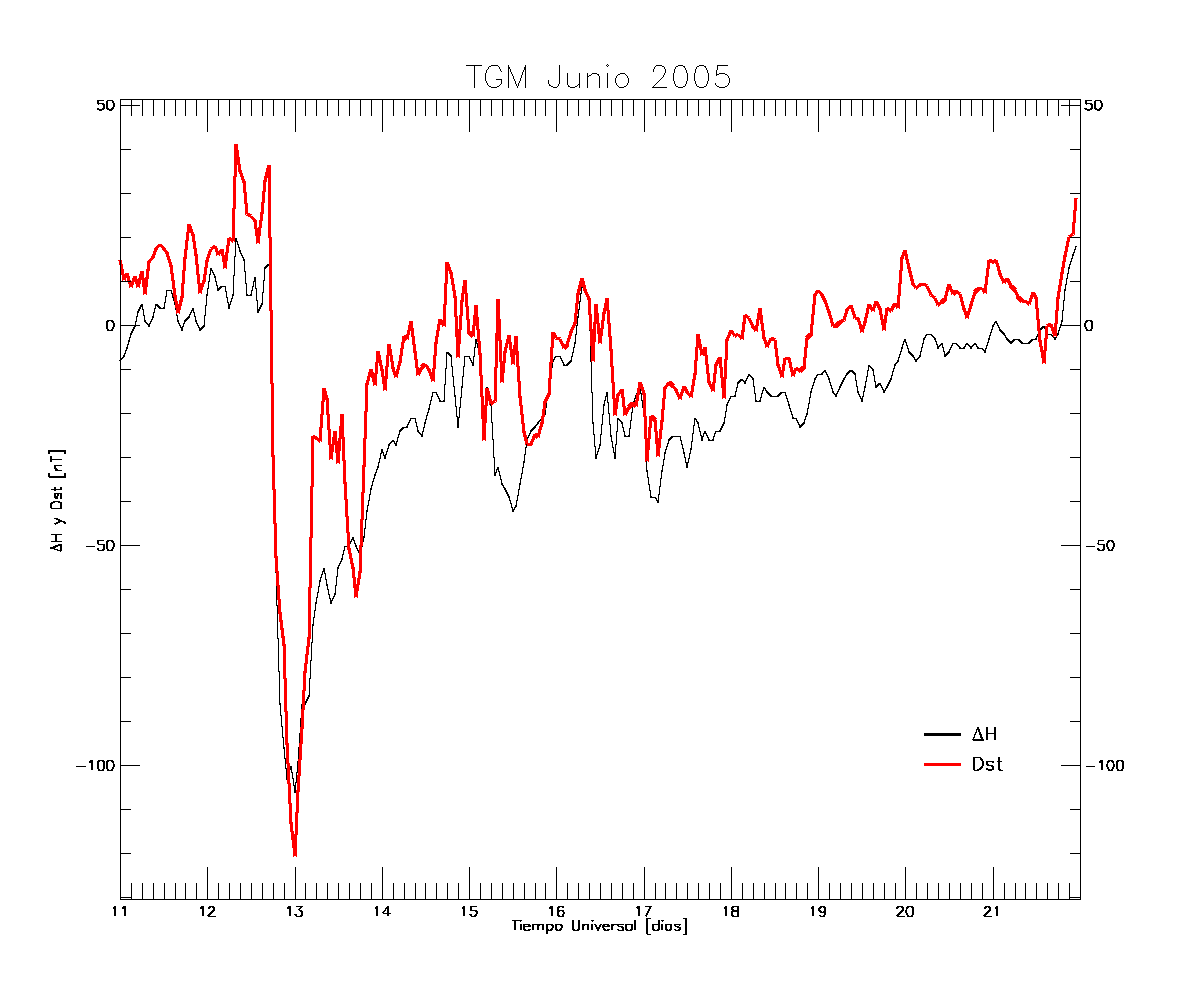
\includegraphics[width=0.32\textwidth]{gmindex2005-06-11_2005-06-21.png}} 
    \subfigure{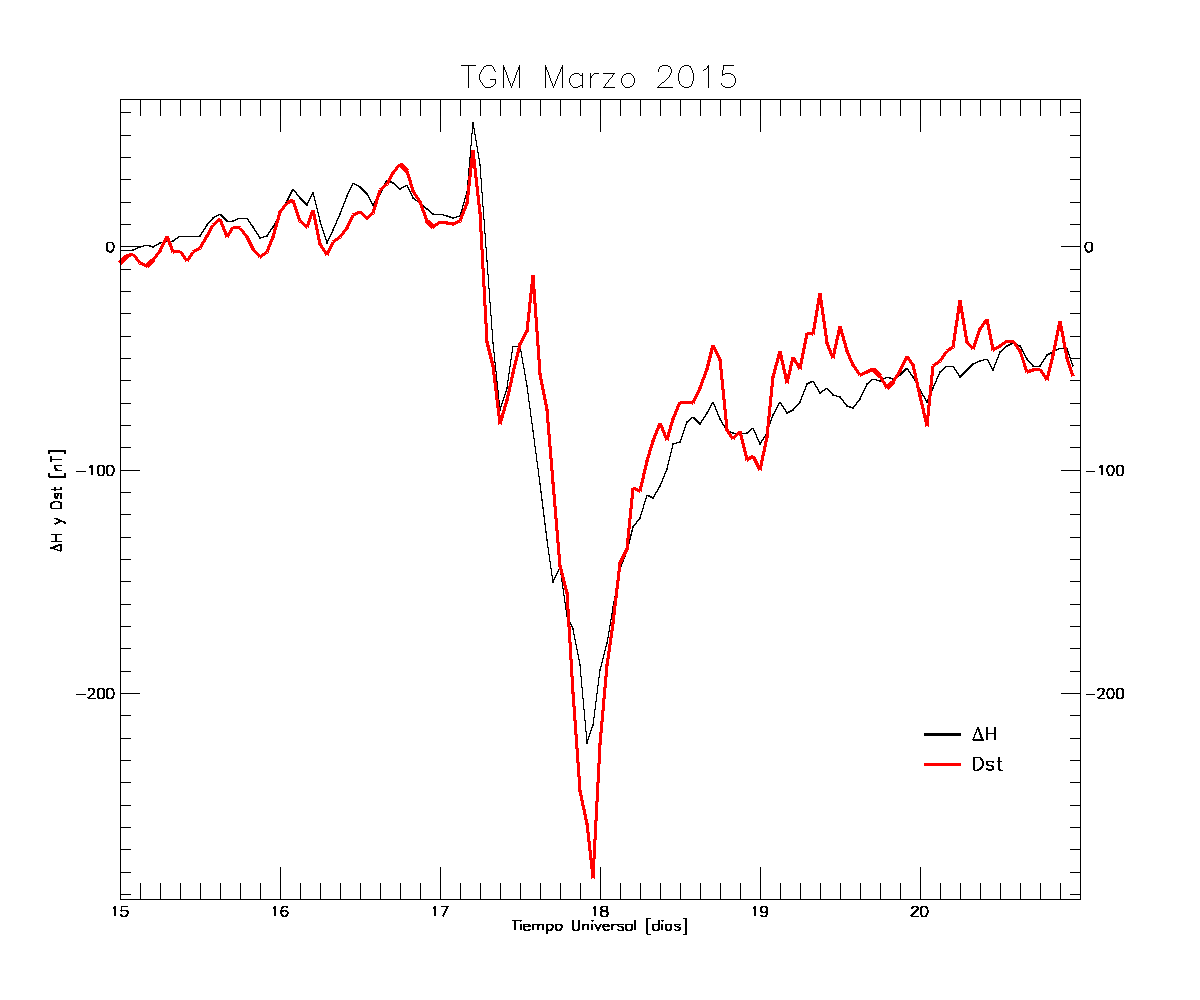
\includegraphics[width=0.32\textwidth]{gmindex2015-03-15_2015-03-20.png}} 
    \subfigure{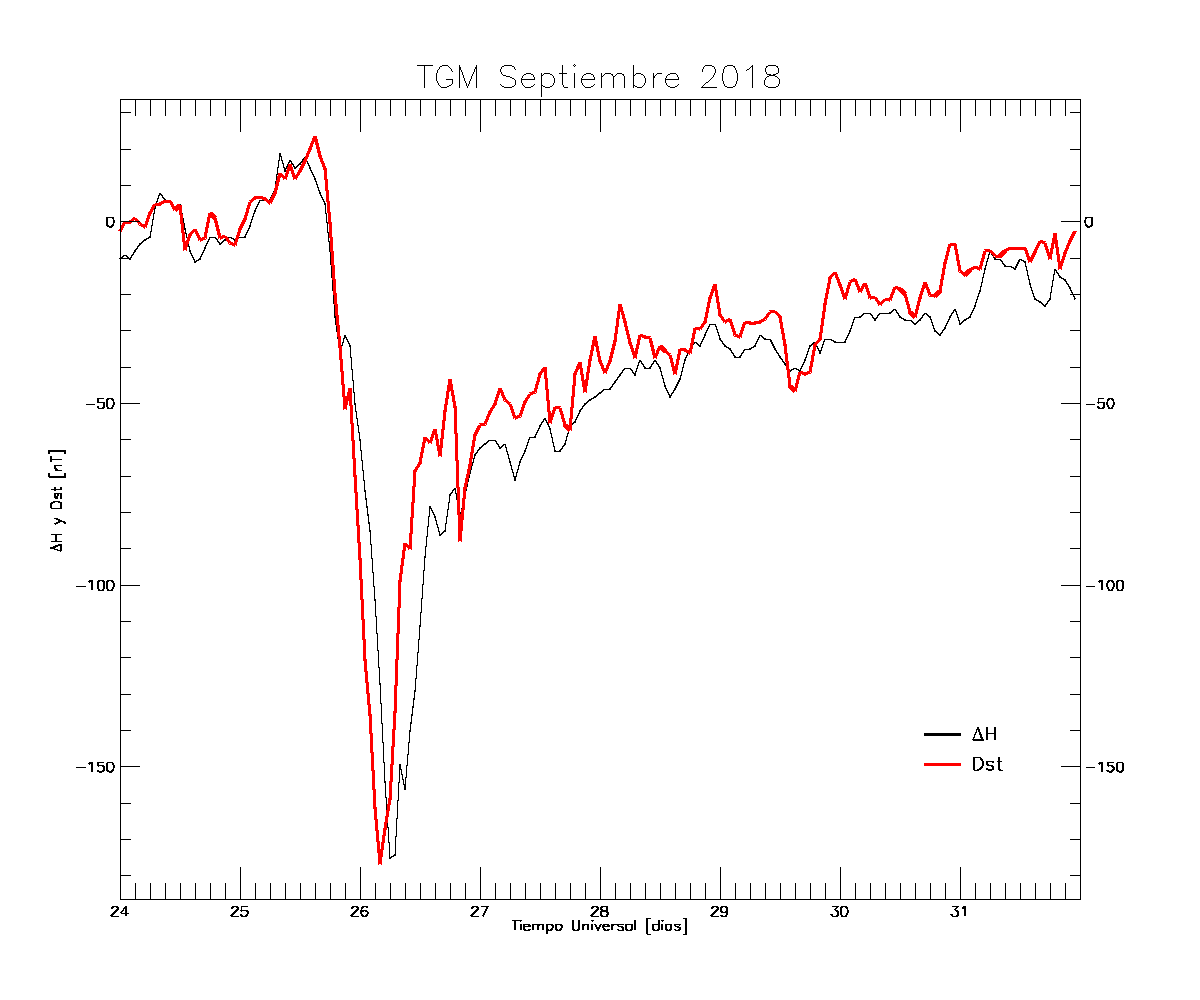
\includegraphics[width=0.32\textwidth]{gmindex2018-08-24_2018-08-31.png}}
    \caption{(left) blah (center) blah (right) blah}
    \label{gse}
\end{figure}

To detect local effects qualitatively, geomagnetic indices can be used throw identifying the differences in time in the geomagnetic response at global and local scales. There are three general differences between the local and planetary geomagnetic responses:  

\begin{enumerate}
    \item     Differences in magnitude 
    \item     Difference in the time response of the main phase 
    \item     Difference in behavior during recovery phase. 
\end{enumerate}

These three cases are observed on the Figure \ref{gse}, however, for a GS, more than one can be applied, depending on the complexity of each event.\\   

The variability on the behavior of a geomagnetic response at a local scale in comparison with the global scale resulting in these 3 different have been studied for a while and their origin can be related to the local time in which the GS is originated, the trigger event and the local ionospheric response.

\section{Results}


\subsection{Local Geomagnetic Effects}

On the Figure \ref{dispersion} the results are showed the comparison in the behavior between $\mathrm{\Delta H}$ and Dst. It is observed that up to –100 nT data points are barely dispersed, keeping a significantly close distance to the diagonal identity which represents a correlation of 1. This is consistent with the correlation of 0.76 for all the Dst inside the range of 100 and –100 nT with their respective $\mathrm{\Delta H}$ values.  On the other hand, during those periods when Dst values went bellow this threshold, begins a more prominent dispersion of the data points. The corresponding correlation for all the values lower than –100 nT decays to 0.63. Of course, these values correspond for the global analysis. As it can be observed in the histogram showed in \ref{hist}, the variation of the correlation in function of the Dst ranges considered has an important fluctuation depending of each GS. \\ 

\begin{figure}
\centering
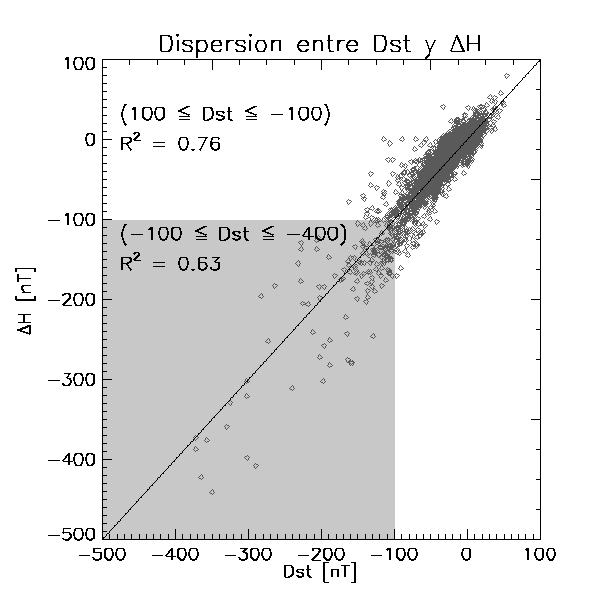
\includegraphics[width=0.8\textwidth]{dispersion_plot.png}
\caption{\label{dispersion}Results from Gradepro}
\end{figure}

These results indicates that the local geomagnetic response has significant differences in comparison to the planetary response, specifically when considering some specific range of Dst and $\mathrm{\Delta H}$ values hence, the evidence suggests the presence of local geomagnetic effects.\\   

\begin{figure}
\centering
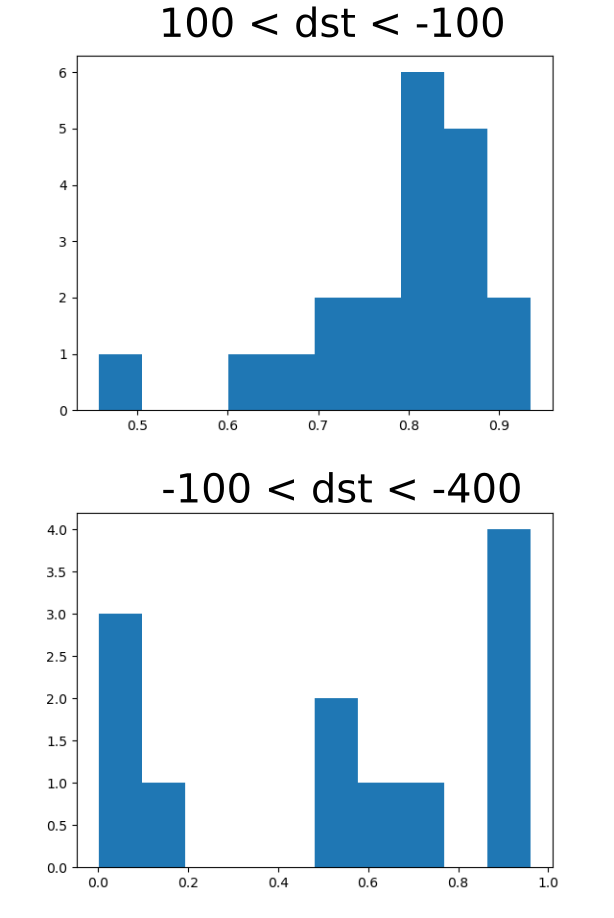
\includegraphics[width=0.5\textwidth]{hist.png}
\caption{\label{hist}Results from Gradepro}
\end{figure}

On the Figure \ref{hist} (Top) it is showed the distribution of the correlations for each event, according to the two ranges previously established. It can be noted that on the first case, there is a clear distribution centered around $R^2 \sim 0.84$, while there is a significant number of cases in which $R^2$ is bellow 0.8. These cases represent about $35\%$ of the study sample. Studying the second range (bottom) there was remarkable difference with respect to the first case: The correlation in general is not just lower but there is more dispersion on the distribution of $R^2$ for each case. Of course, there are events like the GS-2, GS-11 and GS-16 (see the Table \ref{eventstab}) where there is not Dst values bellow –100 nT or the cases GS-8, GS-14, GS-17 and GS-18 where there are not enough number of Dst data points to compute a correct correlation within the range considered. So, the number of cases considered on the second histogram is significantly lower for more detailed distribution analysis with the current number of study cases. \\ 

\begin{figure}
\centering
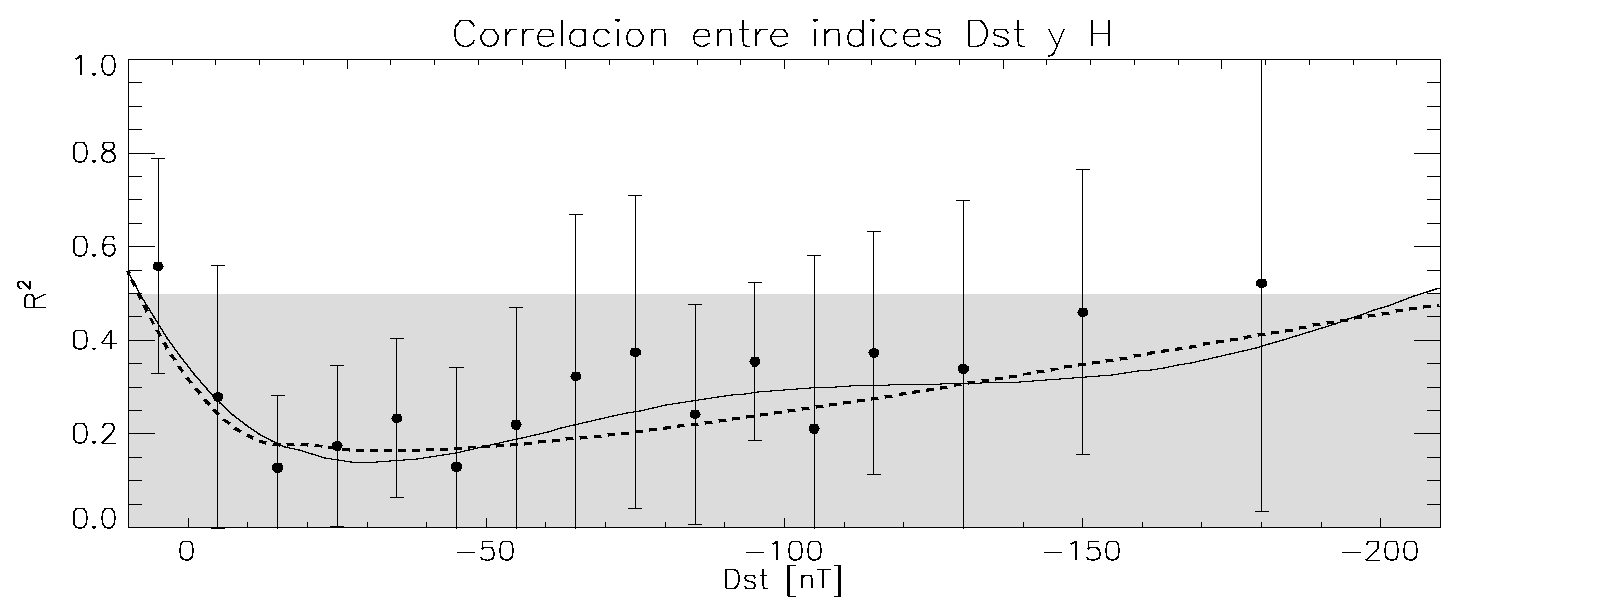
\includegraphics[width=1.0\textwidth]{correlation_plotV4.png}
\caption{\label{correlation}Results from Gradepro}
\end{figure}

To get a better understanding of the relationship between the planetary and local geomagnetic responses, we compute their correlation using the coefficient of determination ($R^2$). We compute $R^2$, considering Dst for ranges of 10 nT from 0 to –140 nT. Considering the decrement in the amount of data with ranges lower, the last ranges were set to be about 20 nT and 40 nT, between –140 and –160, and the last range being between –160 and –400 nT. A second criteria were applied, neglecting those cases in which the number of Dst data points to correlate with were insufficient.\\   

On the Figure \ref{correlation} the results are showed for this analysis. The black circles represent the average of $R^2$ of the 20 GS for each Dst range while the error bars correspond to their standard deviations. The Figure is divided in two regions according to $R^2$. The first region is gray shaded and encompass values from 0 to 0.5 while the region above encompasses values from 0.5 to 1. Those $R^2$ ranges positioned on the top region are considered to have acceptable correlation while the points situated in the shaded area are considered to have lack of correlation. It is important to consider that $R^2$ behavior vary significantly with each event.\\  

Considering a wider number of ranges in this case, allowed us to note a tendency, which is represented with the solid and dashed black lines in the figure. This tendency, at the beginning has a rapid descending until the range of –20 and –50 nT where the we get the minimum $R^2$. For those ranges where Dst goes bellow –50 nT, there is a smooth ascending tendency of $R^2$. Once the general correlation starts to increase we observe that over 0.5 between –150 and –200 nT where Dst and $\mathrm{\Delta H}$ are enough correlated again.\\  

\section{Discussion}

After studying the dispersion of the geomagnetic planetary index with its local equivalent for all the events, we observed two regions are formed: one region closer to the diagonal ($R^2$ = 1.0) and the second region bellow geomagnetic values of –100 nT with a more evident dispersion in the data. The range of values at which dispersion is higher are associated to the main phases of GS. However, considering the behavior of certain GS, it is also expected to have a minor correlation during the recovery phase as we have seen on Figure \ref{gse}. A strong dispersion between local and planetary geomagnetic indices implies a plausible probability of local geomagnetic effects which are responsible for arising these differences. \\ 

Paying attention to the correlation of Dst and $\mathrm{\Delta H}$ allowed to found out an interesting variation in the coefficient $R^2$ for each event. There is a plenty of factors which causes these differences between each event e. g. intensity of the event, the nature of the GS triggers, and the complexity of the GS itself. This can be seen considering the width of the error bars on the Figure \ref{correlation}.\ 

Although there is a considerable variation in $R^2$ for each event, it's important to notice that every case has in common a significant decrease on their correlations on the range between –30 and –60 nT. In this range, the average tendency shows $R^2$ bellow 0.2. Descending under –60 nT it is observed that the average tendency has a smooth growth of $R^2$. \\ 

Initially it was thought that $R^2$ would've descended linearly with the decrement of Dst values however this was not correct at all, because beyond –50 nT the correlation increase. The possible reasons of this are: 

\begin{itemize}
    \item     The reducing of data with each following range limit. 
    \item     The time resolution which is hourly (this could be different for a minute resolution case). 
\end{itemize}

In the case of the stronger events (GS 3 and 6 with Dst < -350 nT) $R^2$ have not a sharp decrease as well as those cases where Dst > -200 nT. The main reason could be because these GS are so intense that the global geomagnetic effects are manifested with quite better uniformity, so this can overshadow the local effects on a specific place. 

\section{Conclusion}
In the present paper we study the differences between the planetary and local geomagnetic response during periods of high geomagnetic activity. In the analysis of the correlation between the planetary and local geomagnetic indices it was found that -30 nT $\leq$ Dst $\leq$ -140 nT, significantly differences in the behavior planetary and local of responses are presented. For Dst values bellow this range, we observed that planetary effects overshadow or ``mask'' partially the local response. Nevertheless, the differences between local and planetary indices represent a local response of the EMF which is independent of the planetary EMF. Consequently, we find evidences of local geomagnetic effects related to GS. \\ 

Analyzing the ionospheric response during those periods when we have more significant differences in the behavior of Dst and $\mathrm{\Delta H}$, we found that such differences concur with local ionospheric disturbances.  \\ 

The differences in the behavior of geomagnetic responses on each scale is attributed to 2 different cases which according to previous studies, depend on (1) local time at which the GS was produced and (2) the local ionospheric which according to [cite] can have a retarding effect and can influence on the local geomagnetic field. \\ 


\subsection*{Guidance: How to add Citations and a References List}

You can upload a \verb|.bib| file containing your BibTeX entries, created with JabRef; or import your \href{https://www.overleaf.com/blog/184}{Mendeley}, CiteULike or Zotero library as a \verb|.bib| file. You can then cite entries from it, like this: \cite{greenwade93}. Just remember to specify a bibliography style, as well as the filename of the \verb|.bib|.

You can find a \href{https://www.overleaf.com/help/97-how-to-include-a-bibliography-using-bibtex}{video tutorial here} to learn more about BibTeX.



\bibliographystyle{alpha}
\bibliography{sample}

\end{document}